\chapter{CIAC}

Para ilustrar melhor como o sistema CIAC irá funcionar será demonstrado alguns cenários com base nas escolhas de algumas variáveis que influenciam diretamente como o CIAC irá se comportar, após isso será descrito em passos o que ocorrerá dando seus resultados e se baseando no caso de uso “Verificar se a ultrapassagem é segura” que se encontra em apêndice. 

Este caso de uso descreve os fluxos possíveis do sistema CIAC e define como é verificado que uma ultrapassagem é segura. 

As variáveis que serão usadas em cada cenário são:

\begin{itemize}
	\item Modelo de cada veículo envolvido na ultrapassagem;
	\item Pista escolhida(Nome da pista, qual local daquela pista, Formato);
	\item Velocidade do veículo que deseja ultrapassar;
	\item Velocidade do veículo que se deseja ultrapassar;
	\item Comprimento do veículo que se deseja ultrapassar;
	\item Velocidade do veículo que vem em sentido oposto a ultrapassagem.
\end{itemize}

\section{Cenário de ultrapassagem simples}

Valor das variáveis:

\begin{itemize}
	\item Modelo dos três veículos envolvidos Gol 1.0 g3/g4;
	\item Pista: BR-262;
	
\begin{figure}[h!]
  \centering
  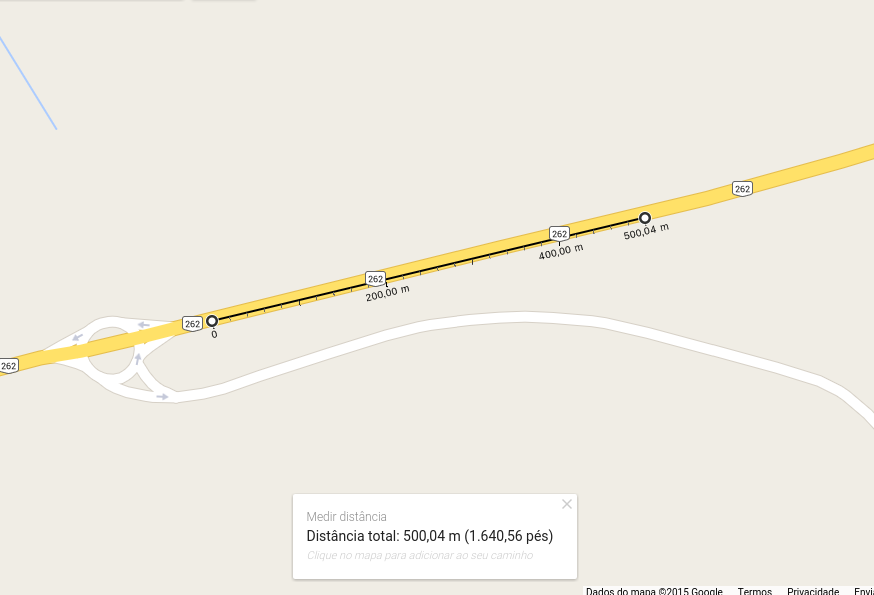
\includegraphics[width=250px, scale=1]{figuras/modelo_pista}
  \caption{Cenário simples}
\label{fig:modelo_pista}
\end{figure}

	\item Início:(-47.668, -19.683) Fim:(-47.662, -19.682);
	\item Tamanho percurso: 0.5 Km;
	\item Velocidade do veículo que deseja ultrapassar: 110 Km/h;
	\item Velocidade do veículo que se deseja ultrapassar: 100 Km/h;
	\item Comprimento do veículo que se deseja ultrapassar: 3.91 m;
	\item Velocidade do veículo que vem em sentido oposto a ultrapassagem: 110 Km/h.
\end{itemize}
	
	
Para facilitar a leitura serão considerados alguns fatos: 

\begin{itemize}
	\item O Carro que deseja ultrapassar será chamado de carro1;
	\item O Carro que será ultrapassado será chamado de carro2;
	\item O Carro que vem em sentido oposto será chamado de carro3.
\end{itemize}

Etapas:

\begin{itemize}
	\item O carro1 se aproxima a 5m do carro2 e indica que deseja ultrapassar;
	\item O sistema verifica se há alguma condição que restringe a ultrapassagem, contatando que é possível;
	\item O carro1 se comunica via transponder com o carro2 e obtém o comprimento (que esta armazenado na memória do sistema do carro2) do carro2 e sua velocidade obtida pelo GPS;
	\item O sistema verifica se há um carro na contramão, contatando que existe um carro na contramão;
	\item O sistema se comunica via transponder com o carro3 e obtém sua posição geográfica e sua velocidade obtidos através do GPS;
	\item O sistema calcula se é possível efetuar uma ultrapassagem segura, e da o sinal verde para a ultrapassagem;
	\item O motorista do carro1 ultrapassa;
	\item Enquanto ele ultrapassa, o sistema continua verificando se é possível ultrapassar, sendo que enquanto ocorre a ultrapassagem nada impede a ultrapassagem;
	\item O motorista termina a ultrapassagem.
\end{itemize}

\section{Justificativa da Escolha da Pista}

A BR 262 é uma rodovia transversal brasileira que liga os estados do Espírito Santo, Minas Gerais, São Paulo e Mato grosso do Sul. Tem início em Vitória (ES) e passa por cidades importantes como Manhuaçu, Belo Horizonte, Araxá, Uberaba, Três Lagoas e Campo Grande. Percorre 999,8 Km no estado de Minas Gerais cortando-o de leste a oeste. Em 2009 apresentou um elevado número de acidentes. Ao todo foram registrados 9.614 acidentes em que 280 pessoas morreram. Somente no percurso entre Belo Horizonte e Governador Valadares houveram 2.975 acidentes, no qual 2.159 ficaram feridas e 138 vieram a óbito. Atualmente já possui trechos duplicados, mas ainda conta com muitos trechos de mão dupla. 

\begin{figure}[h!]
  \centering
  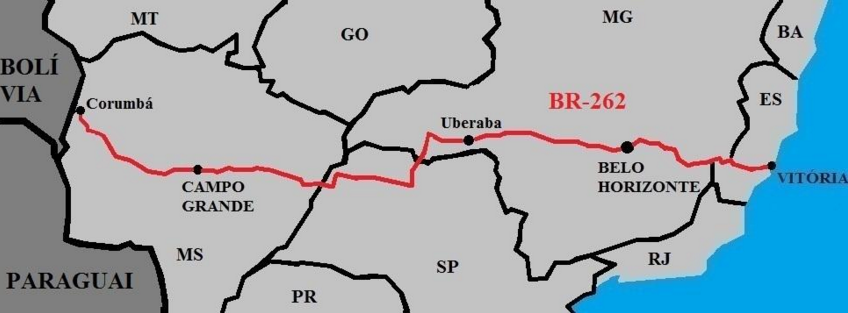
\includegraphics[width=350px, scale=1]{figuras/mapa}
  \caption{Rodovia BR 262}
\label{fig:mapa}
\end{figure}

Em 2014 o Estado de Minas Gerais foi o que apresentou o maior número de acidentes e mortos em rodovias, seguido por Paraná, Santa Catarina, São Paulo e Rio de Janeiro. Essas regiões representam grande parte do contingente populacional do país e, especificamente, o Sudeste responde por 49,5\% do PIB do Brasil, sendo São Paulo, Rio de Janeiro e Minas Gerais, respectivamente, os três estados mais ricos do país. Isso faz com que o fluxo rodoviário nessas regiões seja maior, aumentando o número de acidentes. 

A BR 262 é considerada uma rodovia perigosa, pois apresenta muitos trechos onde a pista é de mão dupla, além de algumas deficiências como a falta de sinalização e condições ruins de tráfego, o que torna necessario a implementação do CIAC. 

\section{Justificativa da Escolha do Modelo do Veículo}

Desde 2007 a Polícia Rodoviário Federal vem fazendo levantamento de dados sobre quais são os veículos que mais se envolvem em acidentes. Em primeiro lugar temos o Volkswagen Gol, que esteve presente em 14.125 acidentes. Em segundo lugar vem o Fiat Uno, envolvido em 8200 acidentes, seguido pelo Fiat Palio, com registro de 7.041 acidentes. 

Sendo assim, foi escolhido o  Volkswagen Gol 1.0 G3/G4, afim de ilustrar o cenário proposto na BR 262.

\begin{figure}[h!]
  \centering
  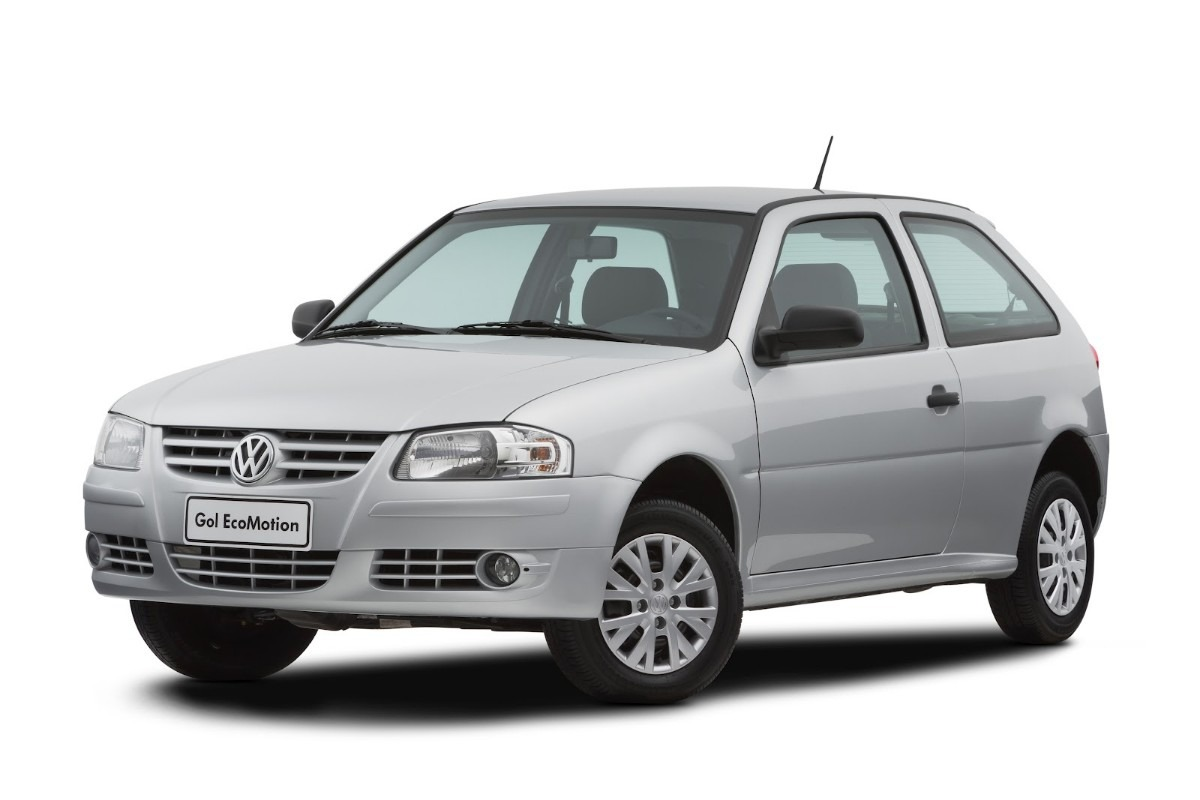
\includegraphics[width=350px, scale=1]{figuras/gol}
  \caption{Volkswagen Gol 1.0 G3/G4}
\label{fig:gol}
\end{figure}





























